\documentclass{article}\usepackage[]{graphicx}\usepackage[]{color}
%% maxwidth is the original width if it is less than linewidth
%% otherwise use linewidth (to make sure the graphics do not exceed the margin)
\makeatletter
\def\maxwidth{ %
  \ifdim\Gin@nat@width>\linewidth
    \linewidth
  \else
    \Gin@nat@width
  \fi
}
\makeatother

\definecolor{fgcolor}{rgb}{0.345, 0.345, 0.345}
\newcommand{\hlnum}[1]{\textcolor[rgb]{0.686,0.059,0.569}{#1}}%
\newcommand{\hlstr}[1]{\textcolor[rgb]{0.192,0.494,0.8}{#1}}%
\newcommand{\hlcom}[1]{\textcolor[rgb]{0.678,0.584,0.686}{\textit{#1}}}%
\newcommand{\hlopt}[1]{\textcolor[rgb]{0,0,0}{#1}}%
\newcommand{\hlstd}[1]{\textcolor[rgb]{0.345,0.345,0.345}{#1}}%
\newcommand{\hlkwa}[1]{\textcolor[rgb]{0.161,0.373,0.58}{\textbf{#1}}}%
\newcommand{\hlkwb}[1]{\textcolor[rgb]{0.69,0.353,0.396}{#1}}%
\newcommand{\hlkwc}[1]{\textcolor[rgb]{0.333,0.667,0.333}{#1}}%
\newcommand{\hlkwd}[1]{\textcolor[rgb]{0.737,0.353,0.396}{\textbf{#1}}}%

\usepackage{framed}
\makeatletter
\newenvironment{kframe}{%
 \def\at@end@of@kframe{}%
 \ifinner\ifhmode%
  \def\at@end@of@kframe{\end{minipage}}%
  \begin{minipage}{\columnwidth}%
 \fi\fi%
 \def\FrameCommand##1{\hskip\@totalleftmargin \hskip-\fboxsep
 \colorbox{shadecolor}{##1}\hskip-\fboxsep
     % There is no \\@totalrightmargin, so:
     \hskip-\linewidth \hskip-\@totalleftmargin \hskip\columnwidth}%
 \MakeFramed {\advance\hsize-\width
   \@totalleftmargin\z@ \linewidth\hsize
   \@setminipage}}%
 {\par\unskip\endMakeFramed%
 \at@end@of@kframe}
\makeatother

\definecolor{shadecolor}{rgb}{.97, .97, .97}
\definecolor{messagecolor}{rgb}{0, 0, 0}
\definecolor{warningcolor}{rgb}{1, 0, 1}
\definecolor{errorcolor}{rgb}{1, 0, 0}
\newenvironment{knitrout}{}{} % an empty environment to be redefined in TeX

\usepackage{alltt}
\IfFileExists{upquote.sty}{\usepackage{upquote}}{}
\begin{document}



\title{HW6 STAT512 Fall2014}

\author{Yet Nguyen}
  
\maketitle


\section*{1.}
\begin{knitrout}
\definecolor{shadecolor}{rgb}{0.969, 0.969, 0.969}\color{fgcolor}\begin{kframe}
\begin{alltt}
\hlkwd{setwd}\hlstd{(}\hlstr{"~/Desktop/tk512/hw6"}\hlstd{)}
\hlstd{dat} \hlkwb{<-} \hlkwd{read.table}\hlstd{(}\hlstr{"HW6_data_2014.txt"}\hlstd{)}
\hlstd{dat[,}\hlnum{1}\hlopt{:}\hlnum{5}\hlstd{][dat[,}\hlnum{1}\hlopt{:}\hlnum{5}\hlstd{]}\hlopt{==}\hlnum{1}\hlstd{]} \hlkwb{<-} \hlopt{-}\hlnum{1}
\hlstd{dat[,}\hlnum{1}\hlopt{:}\hlnum{5}\hlstd{][dat[,}\hlnum{1}\hlopt{:}\hlnum{5}\hlstd{]}\hlopt{==}\hlnum{2}\hlstd{]} \hlkwb{<-} \hlnum{1}
\hlstd{coef} \hlkwb{<-} \hlkwd{summary}\hlstd{(}\hlkwd{lm}\hlstd{(V6}\hlopt{~}\hlstd{V1}\hlopt{*}\hlstd{V2}\hlopt{*}\hlstd{V3}\hlopt{*}\hlstd{V4}\hlopt{*}\hlstd{V5,} \hlkwc{data} \hlstd{= dat))}\hlopt{$}\hlstd{coef[,}\hlnum{1}\hlstd{]}
\hlstd{sort.coef} \hlkwb{<-} \hlkwd{abs}\hlstd{(coef[}\hlkwd{order}\hlstd{(}\hlkwd{abs}\hlstd{(coef))])}
\hlstd{sort.coef}
\end{alltt}
\begin{verbatim}
##          V3:V4          V2:V3       V1:V2:V5       V1:V4:V5 
##       0.003125       0.028125       0.046875       0.053125 
##          V4:V5       V2:V3:V4          V1:V4    V1:V2:V4:V5 
##       0.059375       0.090625       0.103125       0.146875 
##             V1          V2:V5          V2:V4       V2:V4:V5 
##       0.153125       0.178125       0.221875       0.303125 
##             V3    V1:V2:V3:V4       V2:V3:V5             V4 
##       0.309375       0.378125       0.490625       0.546875 
##    V1:V3:V4:V5       V1:V3:V4          V1:V3 V1:V2:V3:V4:V5 
##       0.559375       0.603125       0.609375       0.671875 
##       V1:V2:V4          V1:V5       V3:V4:V5       V1:V2:V3 
##       0.734375       0.746875       0.746875       0.784375 
##    V1:V2:V3:V5    V2:V3:V4:V5       V1:V3:V5             V5 
##       0.815625       0.896875       0.903125       1.034375 
##          V1:V2          V3:V5             V2    (Intercept) 
##       1.190625       1.465625       3.478125      75.321875
\end{verbatim}
\begin{alltt}
\hlstd{n} \hlkwb{<-} \hlnum{31}
\hlstd{p} \hlkwb{<-} \hlnum{1}\hlopt{/}\hlnum{2}\hlopt{+} \hlstd{(}\hlnum{1}\hlopt{:}\hlstd{n}\hlopt{-}\hlnum{1}\hlopt{/}\hlnum{2}\hlstd{)}\hlopt{/}\hlstd{(}\hlnum{2}\hlopt{*}\hlstd{n)}
\hlstd{q} \hlkwb{<-} \hlkwd{qnorm}\hlstd{(p)}
\hlkwd{plot}\hlstd{(q, sort.coef[}\hlopt{-}\hlnum{32}\hlstd{],} \hlkwc{main} \hlstd{=} \hlstr{"haft-normal Plot"}\hlstd{,}
     \hlkwc{xlab} \hlstd{=} \hlstr{"nonnegative normal quantiles"}\hlstd{,}
     \hlkwc{ylab} \hlstd{=} \hlstr{"|estimates|"}\hlstd{)}
\end{alltt}
\end{kframe}

{\centering 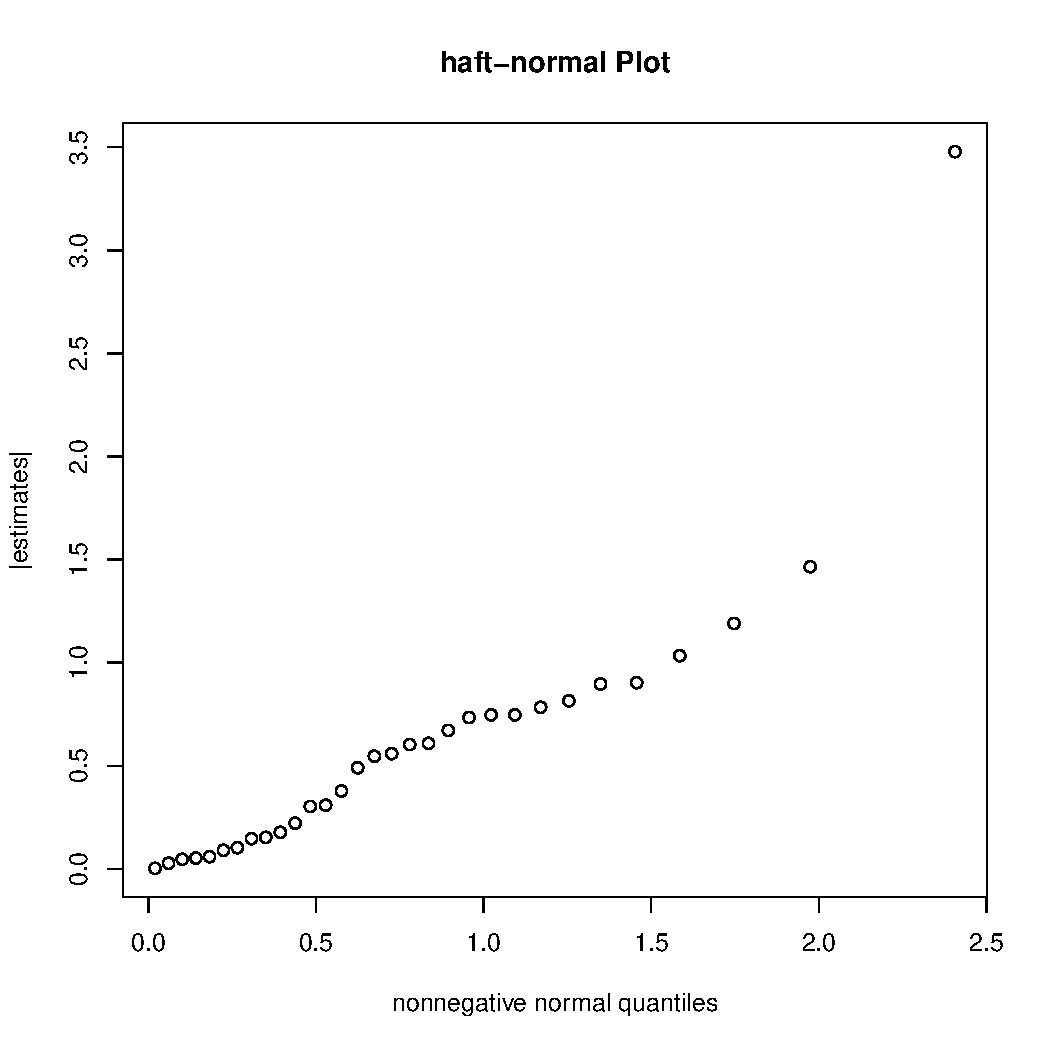
\includegraphics[width=\maxwidth]{figure/minimal-unnamed-chunk-2} 

}



\end{knitrout}
Based on the plot, I think the factorial effects are non-zero are V2, V3:V5.

\section*{2.}
\begin{knitrout}
\definecolor{shadecolor}{rgb}{0.969, 0.969, 0.969}\color{fgcolor}\begin{kframe}
\begin{alltt}
\hlstd{B} \hlkwb{<-} \hlstd{sort.coef[}\hlopt{-}\hlnum{32}\hlstd{]}
\hlcom{# initial robust estimate of sigma/N}
\hlstd{s0} \hlkwb{<-} \hlnum{1.5}\hlopt{*}\hlkwd{median}\hlstd{(B)}
\hlcom{# Let Bs be the subset of B less than 2.5 * s0}
\hlstd{Bs} \hlkwb{<-} \hlstd{B[B}\hlopt{<=}\hlnum{2.5}\hlopt{*}\hlstd{s0]}
\hlcom{# compute the pseudo standard error}
\hlstd{PSE} \hlkwb{<-} \hlnum{1.5} \hlopt{*} \hlkwd{median}\hlstd{(Bs)}
\hlstd{PSE}
\end{alltt}
\begin{verbatim}
## [1] 0.7781
\end{verbatim}
\begin{alltt}
\hlcom{# which coeficients greater  than t*PSE}
\hlstd{t} \hlkwb{<-} \hlnum{1.8}
\hlkwd{which}\hlstd{(B}\hlopt{>=}\hlstd{t}\hlopt{*}\hlstd{PSE)}
\end{alltt}
\begin{verbatim}
## V3:V5    V2 
##    30    31
\end{verbatim}
\end{kframe}
\end{knitrout}

\section*{3.}
If V2 and V3:V5 are included in the model, then 
\begin{itemize}
\item to sastify the hierachy principle,  we need to include factors V3, V5.
\item to sastify the heredity principle, we need to include either V3 or V5.
\end{itemize}
\end{document}
